% SECTION ====================================================================================
\section{Sortieren}
% ============================================================================================

\begin{sectionbox}
\subsection{Laufzeiten von Sortier-Algorithmen}\smallskip
\begin{center}
    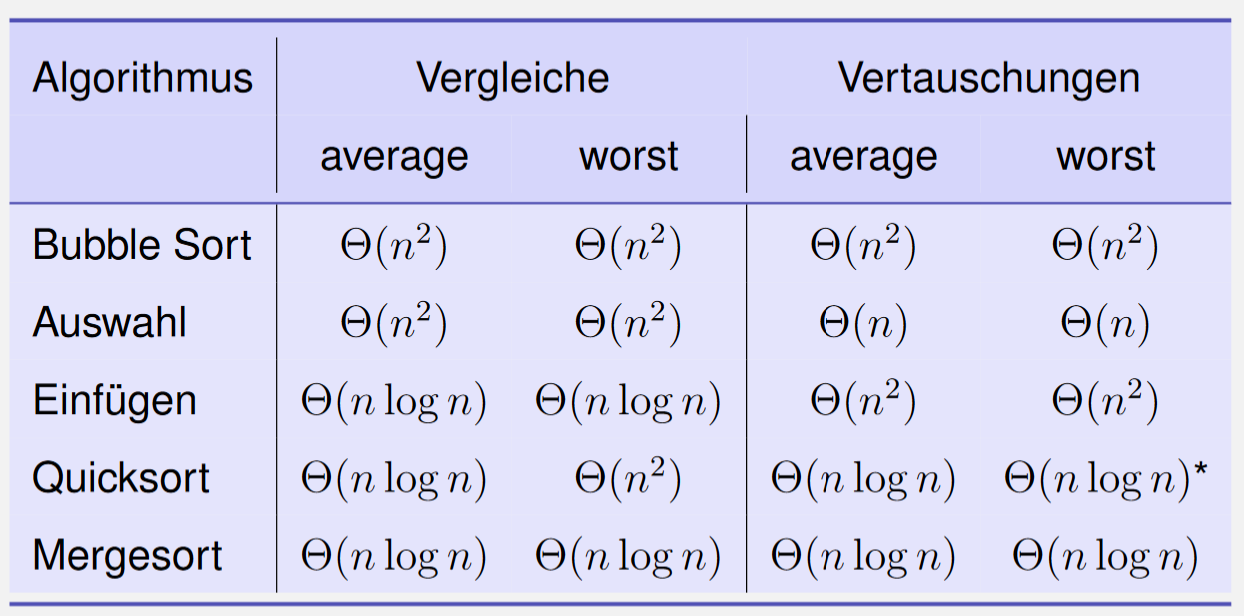
\includegraphics[width = \columnwidth]{../img/LaufzeitenSort.png}
\end{center}
\end{sectionbox}

\begin{sectionbox}
\subsection{Bubble-Sort}
\begin{lstlisting}[language=C++]
void bubbleSort(std::vector<T> vec) { 
    n = vec.size();
    for (unsigned int i = 0; i < n; ++i) {
        for (unsigned int j = 0; j < n - i - 1; ++j) {
            if (vec[j] > vec[j+1]) {
                std::swap(arr[j], arr[j+1]);
            }
}}}
\end{lstlisting}\vspace{-6px}
\end{sectionbox}

\begin{sectionbox}
\subsection{Sortieren durch Auswahl}\smallskip
\begin{tabular*}{\columnwidth}{@{\extracolsep\fill}ll@{}}
\multirow{9}{*}{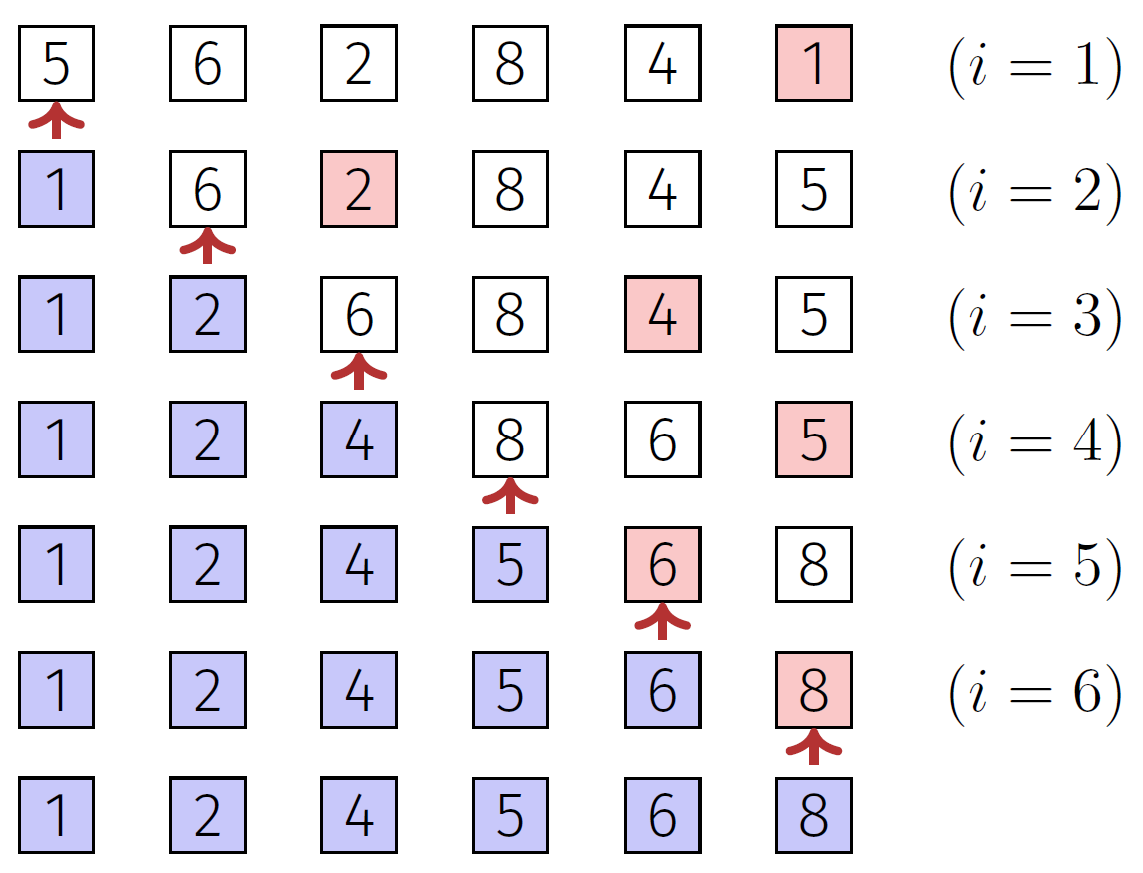
\includegraphics[width = 0.5\columnwidth]{../img/selectSort.png}}
& Auswahl des kleinsten Elementes \\
& durch Suche im unsortierten Teil \\
& A[i:n] des Arrays.\smallskip \\
& Tausche kleinstes Element \\
& an das erste Element des \\
& unsortierten Teiles.\smallskip\\
& Unsortierter Teil wird ein\\
& Element kleiner $(i \rightarrow i+1)$.\\
& Wiederhole bis alles sortiert.\\
\end{tabular*}\smallskip

\textbf{Selection Sort}\par
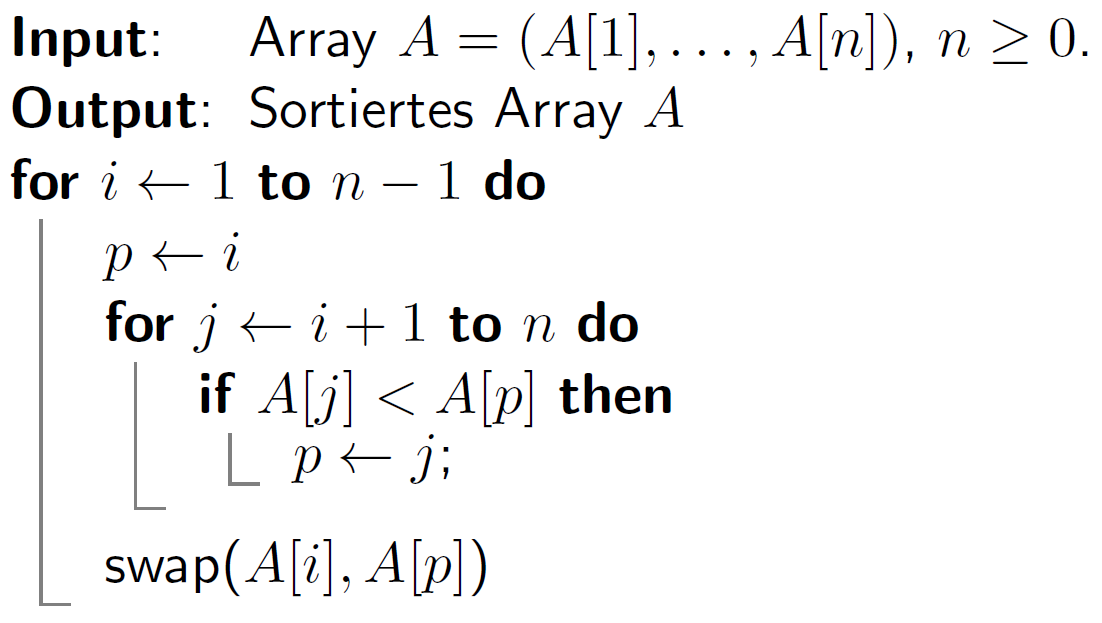
\includegraphics[width = 0.7\columnwidth]{../img/selectSortCode.png}\par\smallskip

\textbf{Analyse}\par
\begin{tabular*}{\columnwidth}{@{\extracolsep\fill}ll@{}}
Anzahl Vergleiche im schlechtesten Fall: & $\Theta(n^{2})$ \\
Anzahl Vertauschungen im schlechtesten Fall: & $n-1=\Theta(n)$\\
\end{tabular*}
\end{sectionbox}

\begin{sectionbox}
\subsection{Sortieren durch Einfügen}\smallskip
\begin{tabular*}{\columnwidth}{@{\extracolsep\fill}ll@{}}
\multirow{7}{*}{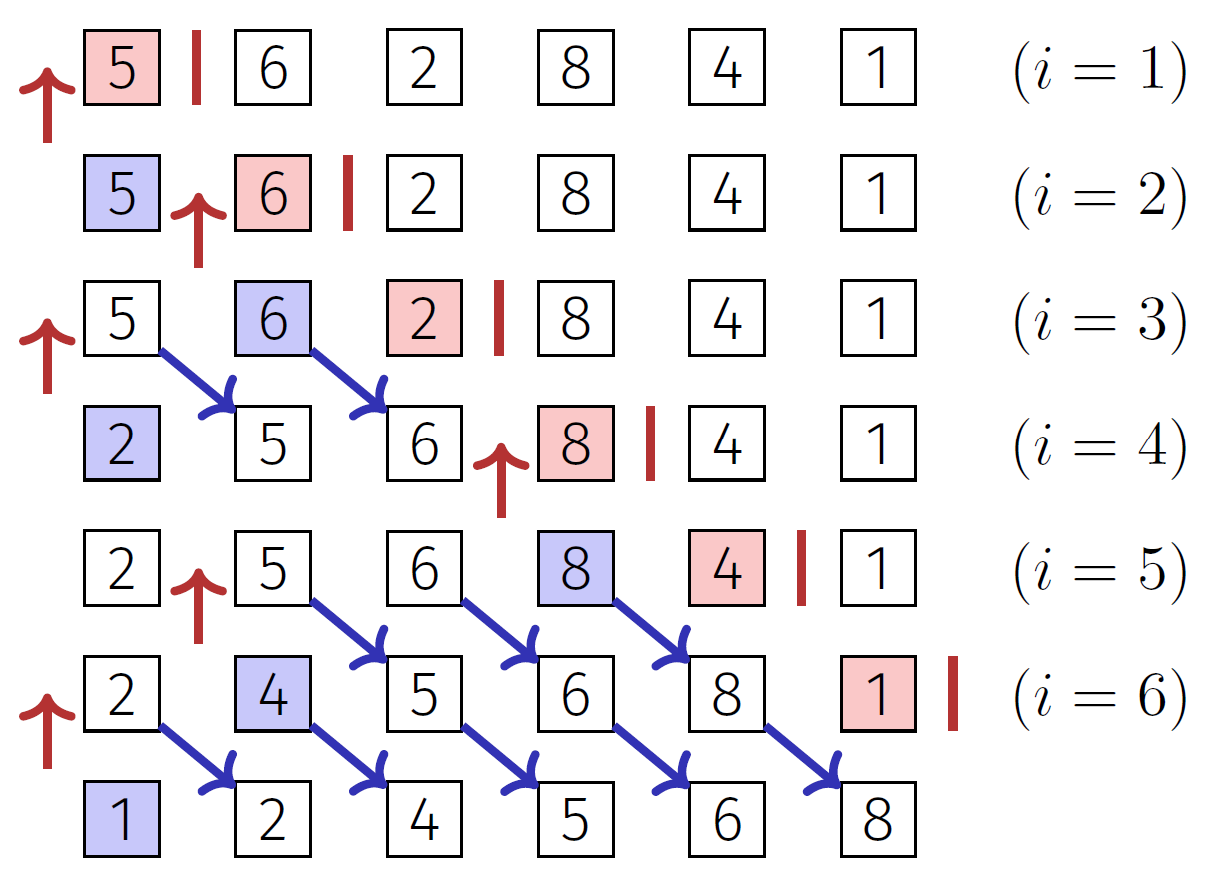
\includegraphics[width = 0.55\columnwidth]{../img/InsSort.png}}
& Iteratives Vorgehen: \\
& $i=1\rightarrow n$ \smallskip \\
& Einfügeposition für \\
& Element $i$ bestimmen. \smallskip\\
& Element $i$ einfügen, ggfs.\\
& Verschiebung nötig. \smallskip\\
& \\
& \\
\end{tabular*}\smallskip

\textbf{Selection Sort}\par
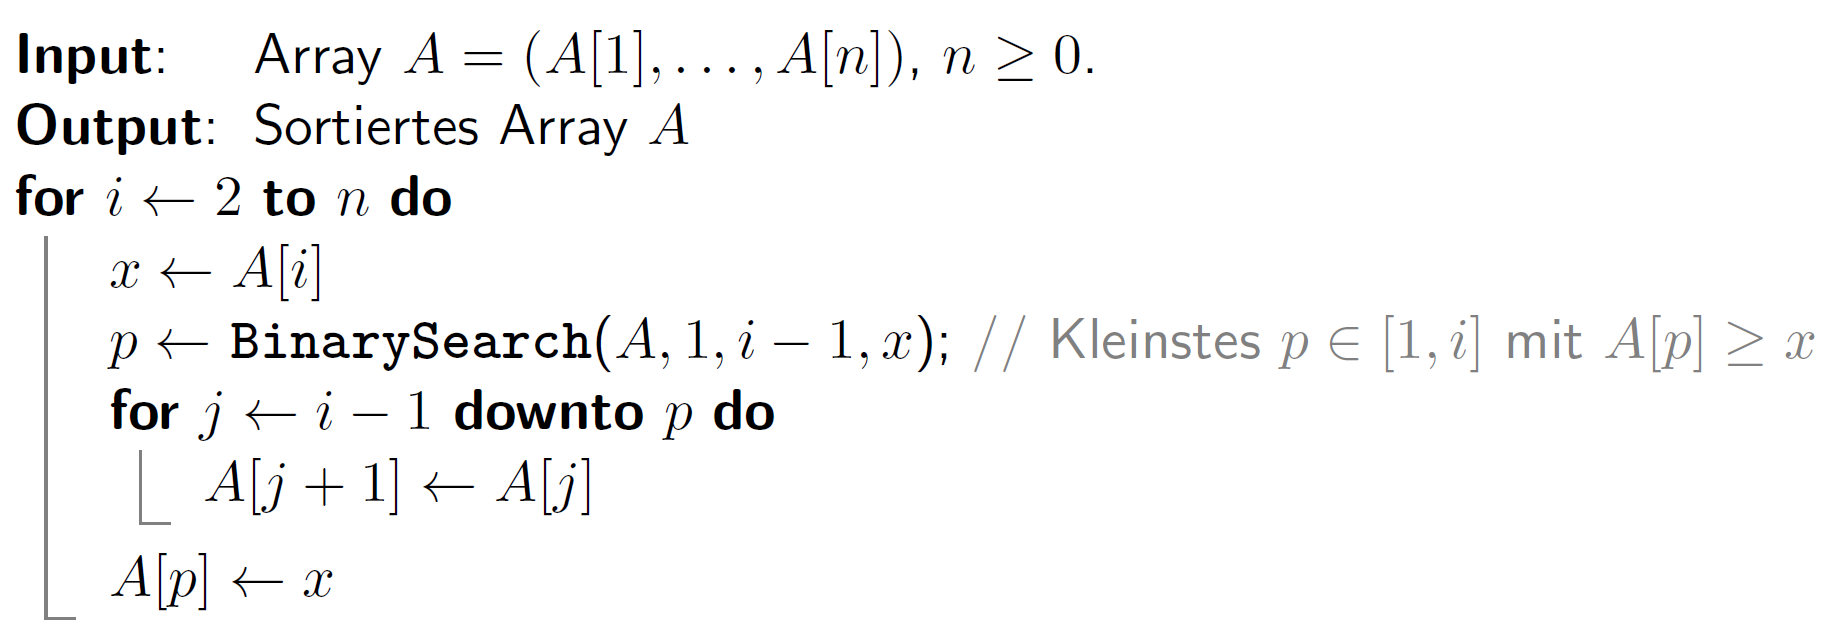
\includegraphics[width = \columnwidth]{../img/InsSortCode.png}\par\smallskip

\textbf{Analyse}\par
Nachteil: Im schlechtesten Fall viele Elementverschiebungen. / Vorteil:  Der Suchbereich (Einfügebereich) ist bereits sortiert $\rightarrow$ binäre Suche möglich.

\end{sectionbox}

\subsection{Mergesort}\smallskip
\begin{sectionbox}
\subsubsection{Merge}\smallskip
Minimum von A kann mit 2 Vergleichen ermittelt werden.\par
\begin{center}
    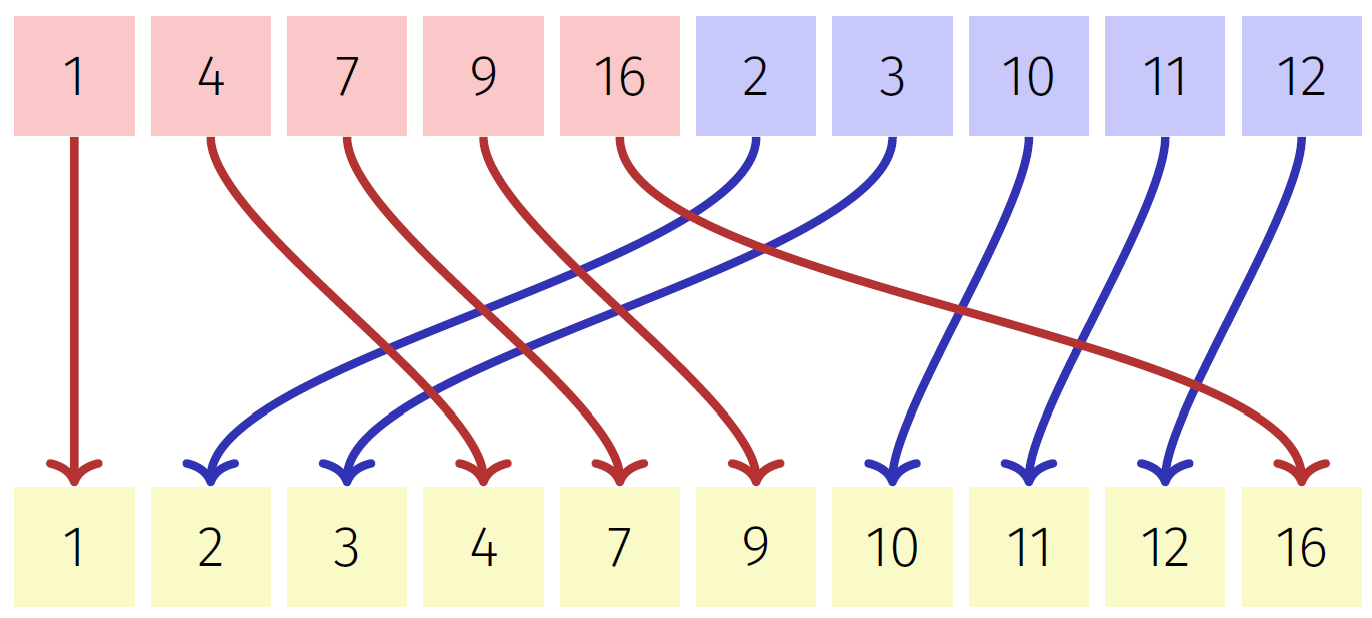
\includegraphics[width = 0.5\columnwidth]{../img/Merge.png}
\end{center}\smallskip
\textbf{Merge(A,l,m,r)}\par
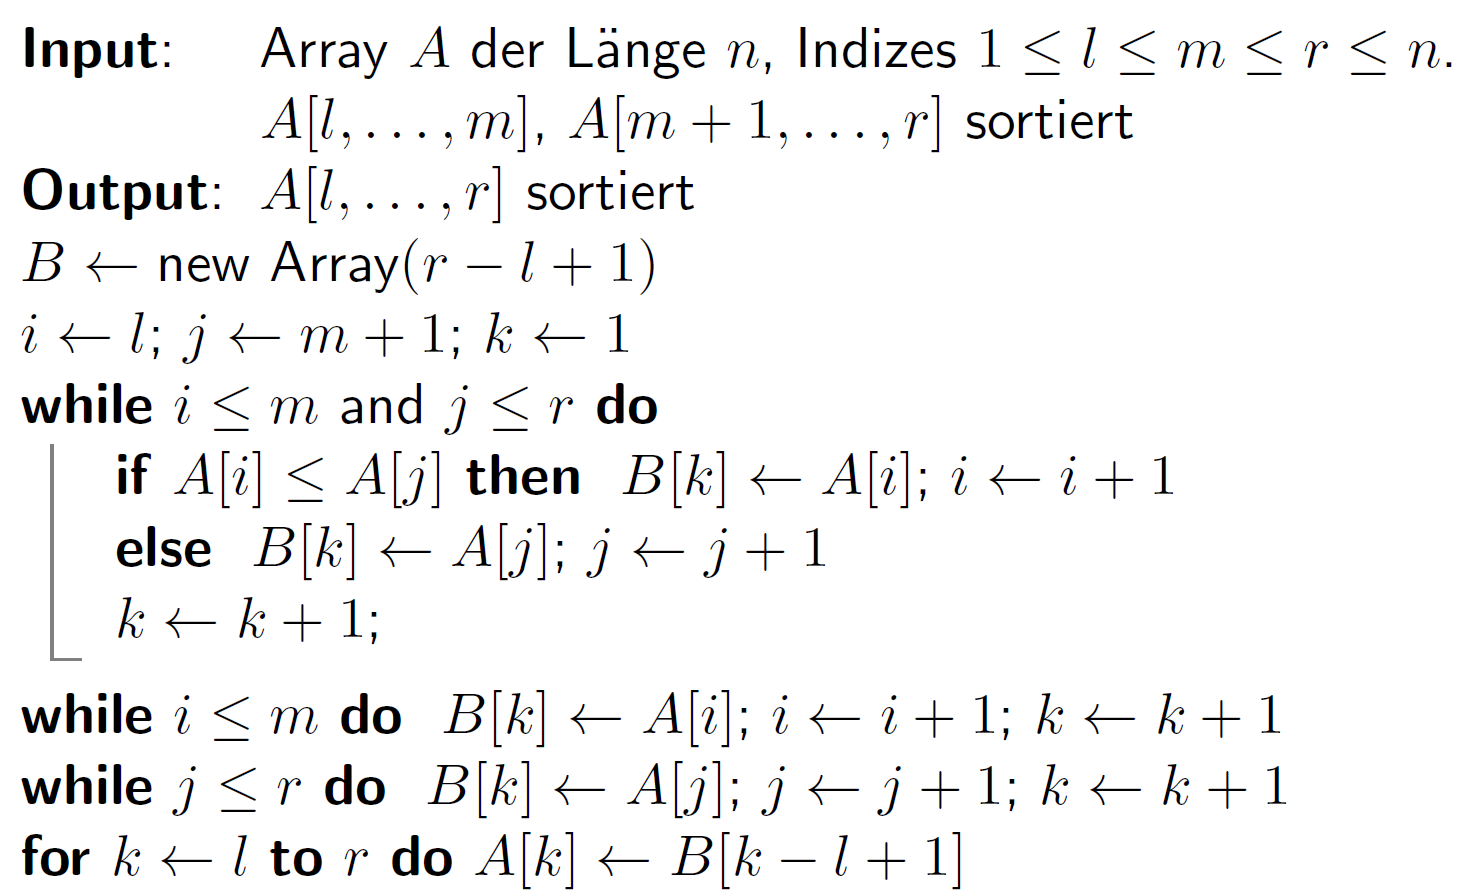
\includegraphics[width = 0.75\columnwidth]{../img/MergeCode.png}
\smallskip
\end{sectionbox}

\begin{sectionbox}
\subsubsection{Mergesort}
\begin{center}
    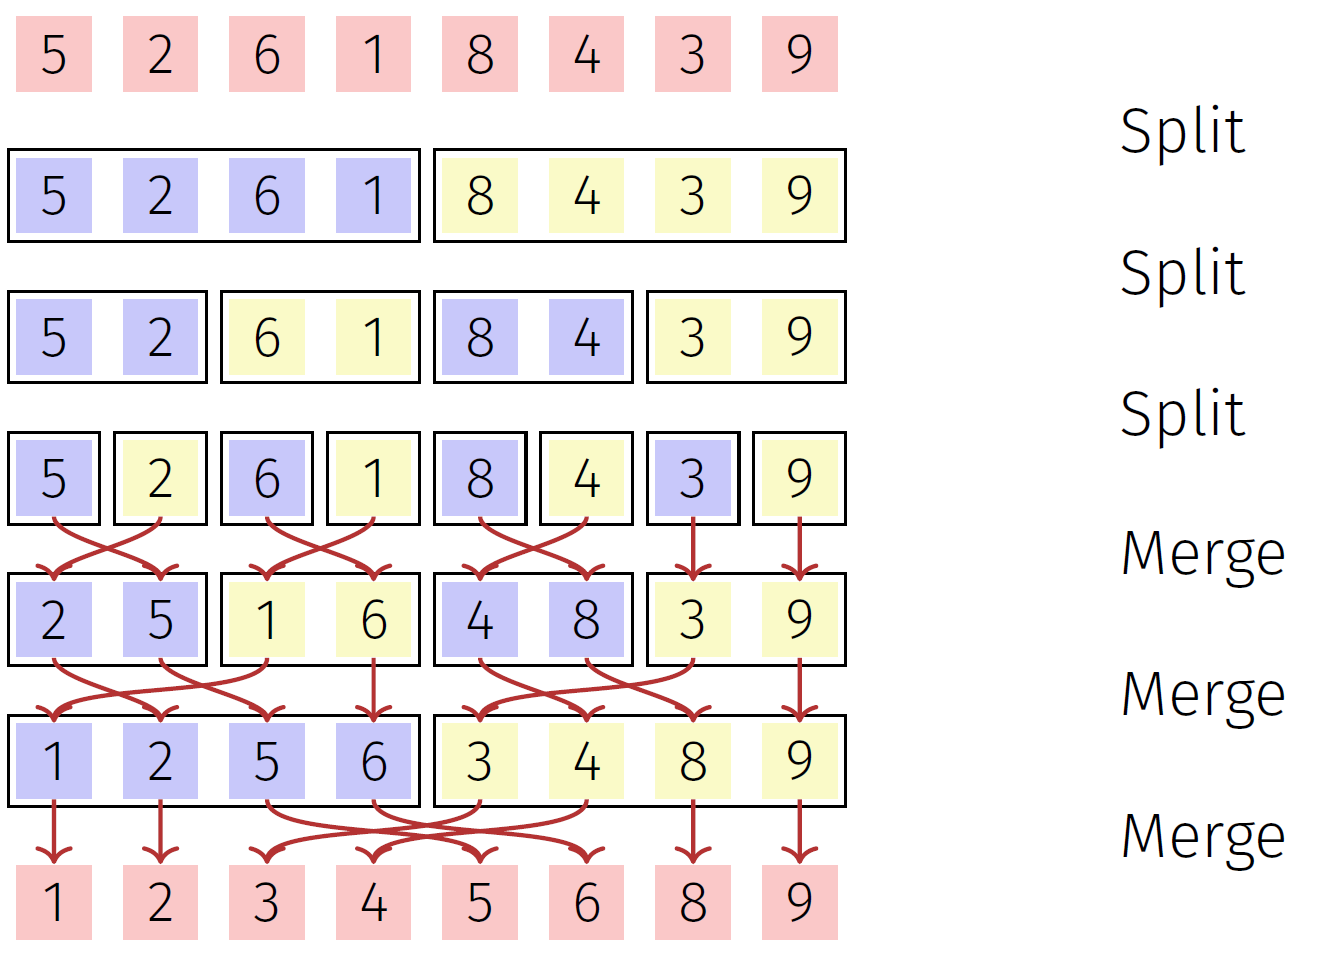
\includegraphics[width = 0.5\columnwidth]{../img/Mergesort.png}
\end{center}\smallskip
\textbf{Mergesort(A,l,r) $\rightarrow$ rekursive Variante}\par
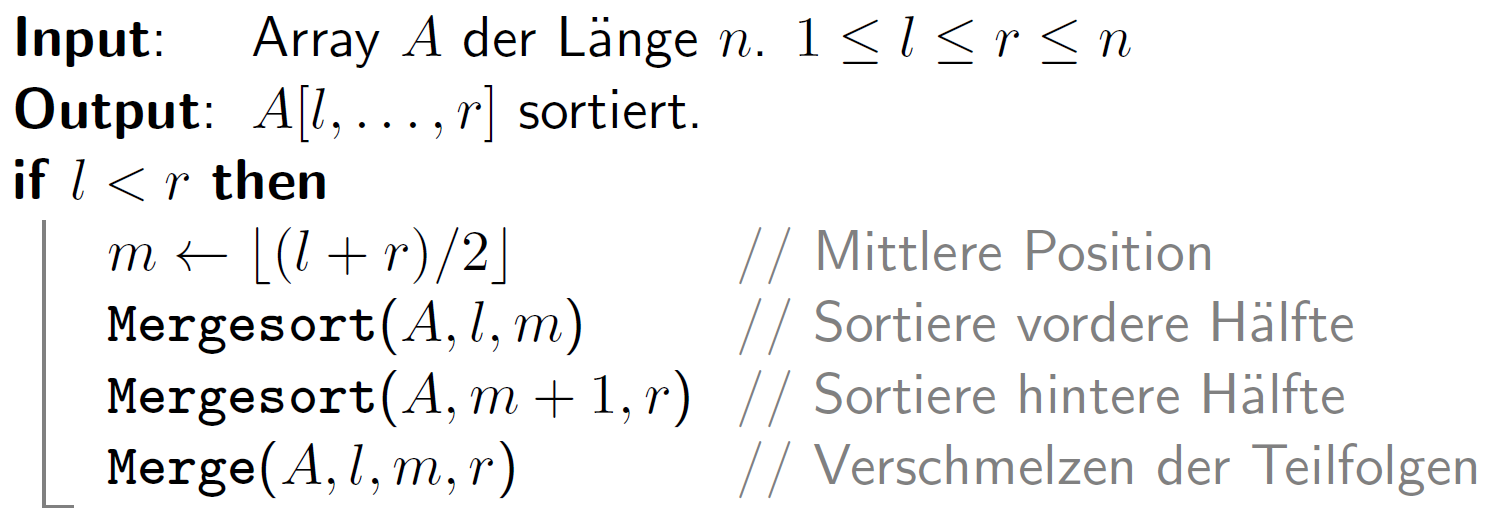
\includegraphics[width = 0.75\columnwidth]{../img/MergesortCode.png}
\par\smallskip
\textbf{Analyse}: Laufzeit  $\Theta(n \operatorname{log}(n))$
\end{sectionbox}

\begin{sectionbox}
\subsection{Quicksort}\smallskip
\textbf{Pivotieren}\par
\begin{enumerate}
    \item Wähle ein beliebiges ELement als Pivot\par
    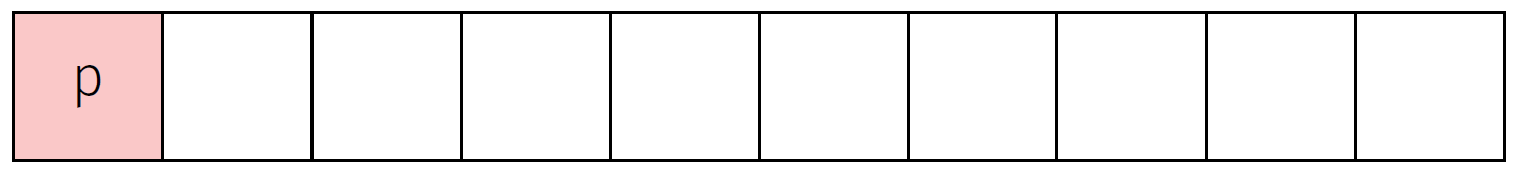
\includegraphics[width = 0.4\columnwidth]{../img/pivot1.png}
    \item Teile A in zwei Teile\par
    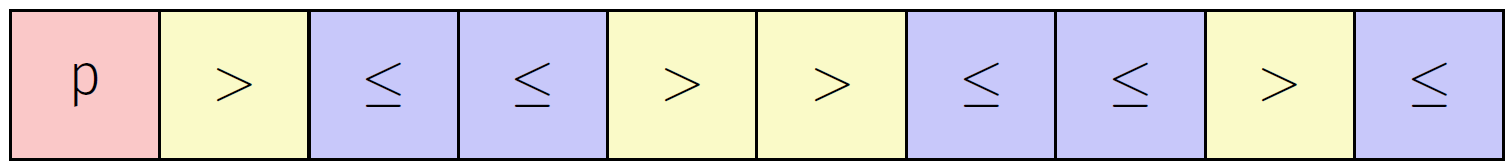
\includegraphics[width = 0.4\columnwidth]{../img/pivot2.png}
    \item Quicksort: Rekursion auf L und R\par
    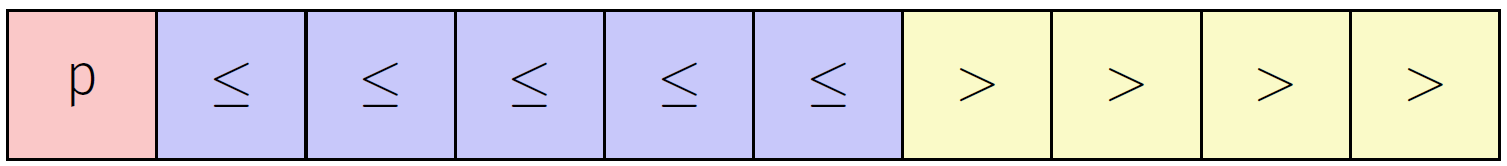
\includegraphics[width = 0.4\columnwidth]{../img/pivot3.png}
    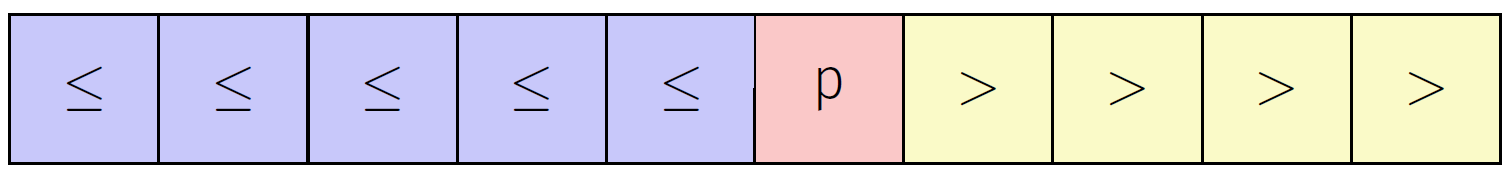
\includegraphics[width = 0.4\columnwidth]{../img/pivot4.png}
\end{enumerate}\smallskip
\textbf{Wahl des Pivot}\par
Maximum/Minimum (worst case) in $\mathcal{O}(n^{2})$.\par
Best case (Pivot in der Mitte) $\omega(n)$.\par\smallskip
\textbf{Partition(A,l,r,p)}\par
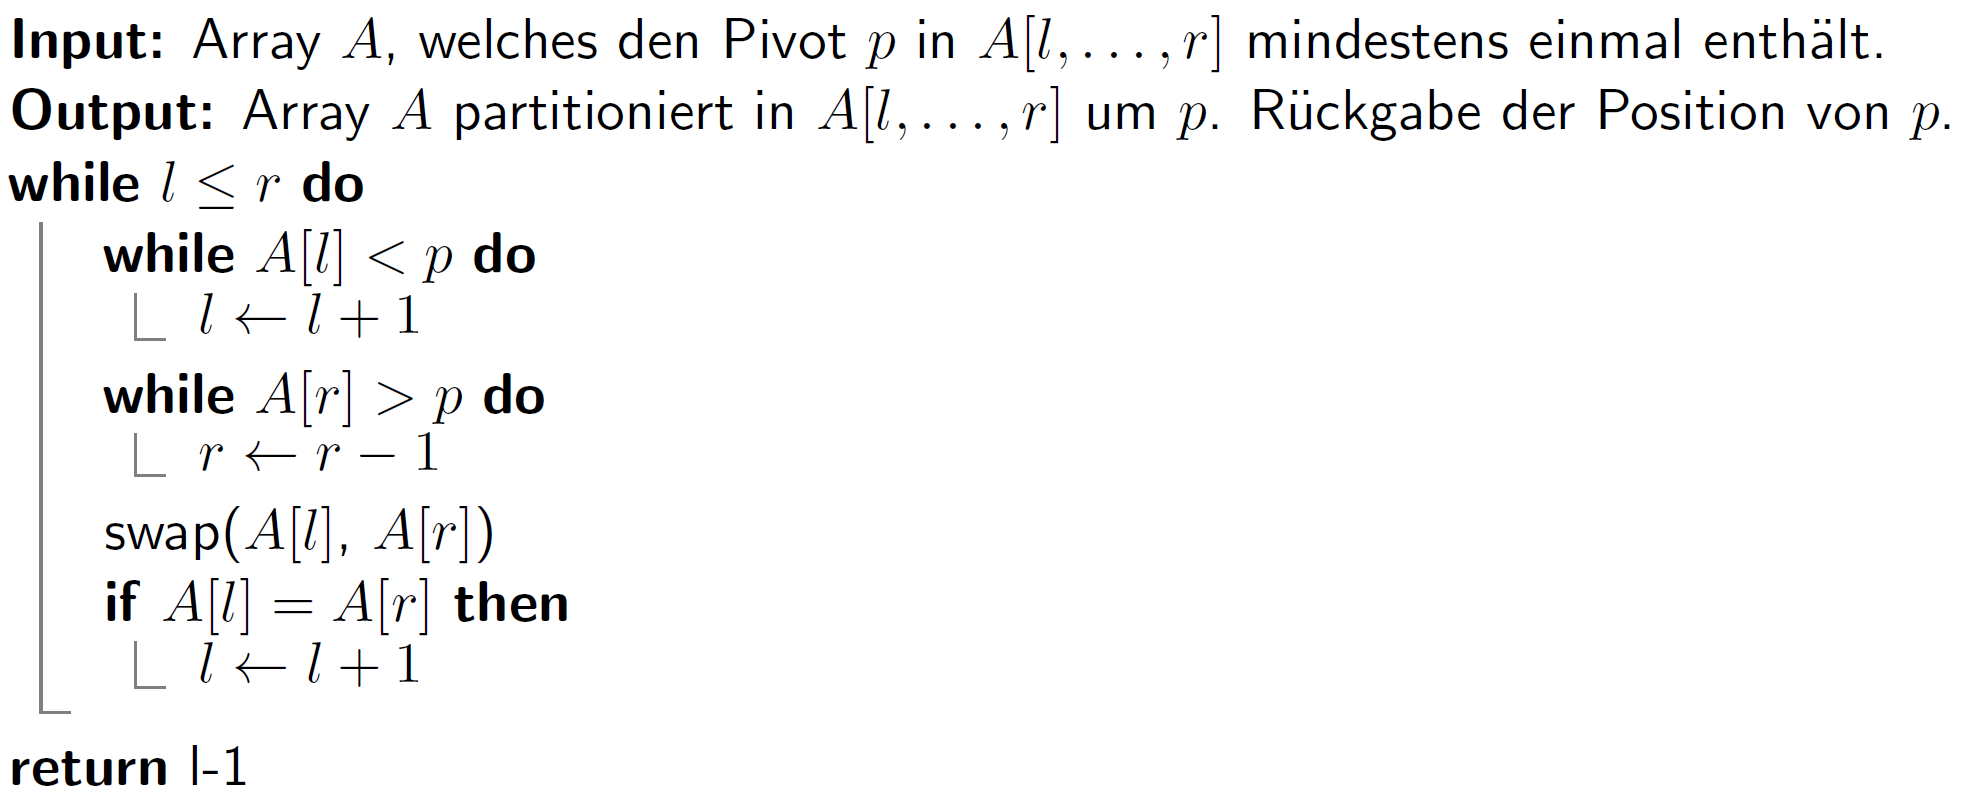
\includegraphics[width = \columnwidth]{../img/PartCode.png}
\par\smallskip

\textbf{Quicksort(A,l,r)}\par
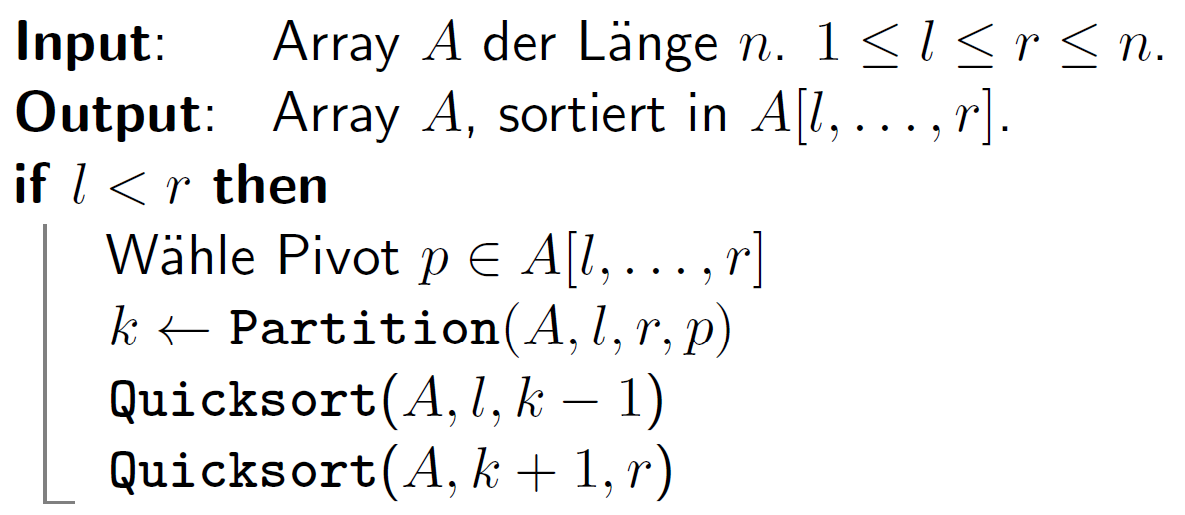
\includegraphics[width = 0.8\columnwidth]{../img/QuicksortCode.png}
\par\smallskip
\begin{greenbox}
Im Mittel benötigt randomisiertes Quicksort $\mathcal{O}(n \cdot \operatorname{log}(n))$ Vergleiche.
\end{greenbox}
\end{sectionbox}

\vspace{36px}